\documentclass{article}
\usepackage[utf8]{inputenc}
\usepackage[russian]{babel}
\usepackage{amsfonts} 
\usepackage{graphicx}
\usepackage{indentfirst}
\usepackage[export]{adjustbox}[2011/08/13]
\usepackage{amsmath}
\usepackage{sectsty}
\sectionfont{\centering}
\makeatletter
\renewcommand*\env@matrix[1][*\c@MaxMatrixCols c]{%
  \hskip -\arraycolsep
  \let\@ifnextchar\new@ifnextchar
  \array{#1}}
\makeatother

\title{Теория кодирования. \\ Конспект практических занятий}
\author{Ерофей Башунов}
\date{}

\begin{document}

\maketitle

\newpage
\section*{3 сентября 2021}

\subsection*{Линейные коды}

Допустим, у нас есть некоторое векторное $n$-мерное пространство $\mathbb{F}^n_q$, где $q$ --- количество элементов. Выберем подпространство размерности $k$ ($n > k$), это и будет являться линейным кодом размерности $n$ и ранга $k$. Параметр $q$ отвечает за арность кода (при $q = 2$ код является бинарным).

Отображение из $k$ бит в $n$ бит --- добавление избыточной информации к векторам из подпространства. Это отображение необходимо для того, чтобы повысить устойчивость передачи информации к помехам путём добавления дополнительных ($n - k)$ <<проверяющих>> битов. Формально, оно записывается в виде $\mathbb{F}^k_q \rightarrow \mathbb{F}^n_q$.

Рассмотрим два вектора таких, что $a \in \mathbb{F}^k_q $ и $c \in \mathbb{F}^n_q$. Тогда преобразование можно рассматривать как умножение вектора на матрицу, а именно:

$$c = a \cdot \underset{k \times n}{G}$$

Матрица $G$ называется порождающей матрицей.

\subsection*{Проверочная матрица}

Проверочная матрица $H^T$ --- способ определить, является ли слово кодовым или нет. Необходимое и достаточное условие: $c \cdot H^T = 0$. Матрица находится с помощью уравнения:

$$\underset{k \times n}{G} \cdot \underset{n \times (n - k)}{H^T} = 0$$

Чтобы найти матрицу $H^T$, необходимо выполнить следующий алгоритм:
\begin{enumerate}
    \item Путём линейных преобразований, приводим матрицу $G$ к такому виду, чтобы в левой её части получилась единичная матрица. В процессе преобразований возможна перестановка столбцов (назовём матрицу перестановки $P$). Получится некоторая матрица $G' = G \cdot P$.
    \item Найдём матрицу $H'$ такую, что $G' \cdot H'^T = 0$. Пользуясь тем, что $G' = [I_k | S]$, получаем, что $H' = [-S^T | I_k]$
    \item Так как $(G \cdot P) \cdot (P^{-1} \cdot H^T) = G \cdot H^T = 0$ и $(G \cdot P) \cdot H'^T = G'^T \cdot H'^T = 0$, то верно равенство $H'^T = P^{-1} \cdot H^T$, следовательно $H = H' \cdot P$.
\end{enumerate}

\subsubsection*{Пример}

Допустим, у нас есть матрица $G$ вида

\begin{equation*}
\begin{pmatrix}
1 & 1 & 1 & 1 & 1 & 1 & 1 & 1 \\
1 & 1 & 1 & 1 & 0 & 0 & 0 & 0 \\
1 & 1 & 0 & 0 & 1 & 1 & 0 & 0 \\
1 & 0 & 1 & 0 & 1 & 0 & 1 & 0 \\
\end{pmatrix}
\end{equation*}

Путём линейных образований и перестановки 4 и 5 столбцов получаем матрицу $G'$:

\begin{equation*}
\begin{pmatrix}
1 & 0 & 0 & 0 & 1 & 1 & 1 & 0 \\
0 & 1 & 0 & 0 & 1 & 1 & 0 & 1 \\
0 & 0 & 1 & 0 & 1 & 0 & 1 & 1 \\
0 & 0 & 0 & 1 & 0 & 1 & 1 & 1 \\
\end{pmatrix}
\end{equation*}

Отсюда находим матрицу $H'$ как

\begin{equation*}
\begin{pmatrix}
0 & 0 & 0 & 1 & 1 & 0 & 0 & 0 \\
0 & 0 & 1 & 0 & 0 & 1 & 0 & 0 \\
0 & 1 & 0 & 0 & 0 & 0 & 1 & 0 \\
1 & 0 & 0 & 0 & 0 & 0 & 0 & 1 \\
\end{pmatrix}
\end{equation*}

А матрица $H$ будет иметь вид:

\begin{equation*}
\begin{pmatrix}
1 & 1 & 1 & 1 & 0 & 0 & 0 & 0 \\
1 & 1 & 0 & 0 & 1 & 1 & 0 & 0 \\
1 & 0 & 1 & 0 & 1 & 0 & 1 & 0 \\
0 & 1 & 1 & 0 & 1 & 0 & 0 & 1 \\
\end{pmatrix}
\end{equation*}

\subsection*{Логарифмическое отношение правдоподобия}

$$p(x) \cdot p(y | x) = p(x ^ y) = p(x | y) \cdot p(y)$$
$$p(x | y) = \frac{p(x) \cdot p(y | x)}{p(y)}$$

Выведем формулу логарифмического отношения правдоподобия. Помним, что $p(y | x) = \frac{1}{\sqrt{2 \pi \sigma^2}} \cdot \exp{-\frac{(y - x)^2}{2\sigma^2}}$

\begin{equation*}
\begin{gathered}
L = \log\frac{P(c_i = 0 | y_i)}{P(c_i = 1 | y_i)} = \log{\frac{\frac{1}{2} \cdot \frac{1}{\sqrt{2 \pi \sigma^2}} \cdot \exp{-\frac{(y_i + 1)^2}{2\sigma^2}}}{p(y_i)} \cdot \frac{p(y_i)}{\frac{1}{2} \cdot \frac{1}{\sqrt{2 \pi \sigma^2}} \cdot \exp{-\frac{(y_i - 1)^2}{2\sigma^2}}}} =\\= \log{\exp{\frac{(y_i - 1)^2 - (y_i + 1)^2}{2\sigma^2}}} = \frac{(y_i - 1)^2 - (y_i + 1)^2}{2\sigma^2} = -\frac{4 y_i}{2\sigma^2} = -\frac{2y_i}{\sigma^2}
\end{gathered}
\end{equation*}

\newpage
\section*{10 сентября 2021}

\subsection*{Двоичный симметричный код}

У нас есть двоичный симметричный код длины $n$, исправляющий $t$ ошибок. Вероятность ошибки составляет $p$.

Модель двоичного симметричного кода описывается схемой Бернулли, поэтому имеем формулу для вероятности наличия ошибок при декодировании $n$ бит:

$$P(n) = \sum_{i = t + 1}^{n} C_i^n p^i (1-p)^{n - i}$$

\subsection*{Граница Синглтона для линейных кодов}

Теорема о границе Синглтона: Если код длины $n$ над $q$-ичным полем, а минимальное расстояние между кодами равно $d$, то максимальная мощность такого кода составляет $q^{n - d + 1}$.

\subsection*{Теорема о связи критериев экстремумов по отношению правдоподобия}

Докажем, что максимизация по расстоянию Хэмминга эквивалентна минимизации в метрике Евклида:

$$\max_{c \in C}P(y | c) = \min_{c \in C}\sum(y_i - x_i)^2$$

Доказательство.

\begin{equation*}
\begin{gathered}
\max_{c \in C} P(y | c) = \max_{c \in C} \prod_{i = 0}^{n- 1} p(y_i | c_i) = \max_{c \in C} \prod_{i = 0}^{n- 1} \frac{\exp{-\frac{(y_i - x_i)^2}{2\sigma^2}}}{\sqrt{s \pi \sigma^2}} \sim \\ \sim - \max_{c \in C} \sum_{i = 0}^{n - 1} \frac{(y_i)^2}{2\sigma^2} \sim \min_{c \in C} \sum_{i = 0}^{n - 1} (y_i - x_i)^2
\end{gathered}
\end{equation*}

\subsection*{Ещё одно интересное утверждение о двоичных кодах}

Если у нас есть двоичный код длины $n$ размерности $k$, то количество кодовых слов из этого кода, где на $с_i = 1$ либо $0$, либо $2^{k - 1}$.

Рассмотрим ситуацию, где $c_i > 0$. Если слов, где $c_i = 0$ больше половины, то мы можем прибавить к этим кодам 1 и получить так же больше половины других кодов (что невозможно). Аналогично, если слов, где $c_i = 1$ так же не может быть больше половины. Следовательно, таких слов будет ровно половина, т.е. $\frac{2^k}{2} = 2^{k - 1}$.

\subsection*{Функция Адамара}

Есть функция $f: \mathbb{F}_2^n \rightarrow \mathbb{R}$. Есть функция Адамара высшего порядка $\hat{f}(u) = \sum_{v \in \mathbb{F}_2^n}(-1)^{uv} \cdot f(v)$. Тогда выполняется следующее утверждение:

$$\sum_{u \in C_{\bot}} f(u) = \frac{1}{|C|} \sum_{u \in C} \hat{f}(u)$$.

Пояснение: $C_\bot$ --- дуальный код для $C$.

Доказательство

\begin{equation*}
\begin{gathered}
\frac{1}{|C|} \sum_{u \in C} \hat{f}(u) = \frac{1}{|C|} \sum_{u \in C} \sum_{v \in \mathbb{F}_2^n} (-1)^{<u, v>} f(v) = \frac{1}{|C|} \sum_{v \in \mathbb{F}_2^n} f(v) \sum_{u \in C}  (-1)^{<u, v>} = \\
= \frac{1}{|C|} \left( \sum_{v \in C_\bot} f(v) |C| + \sum_{v \in \mathbb{F}_2^n \setminus C_\bot} f(v) \sum_{u \in C}  (-1)^{<u, v>} \right) = \\
= \frac{\sum_{v \in C_\bot} f(v) |C|}{|C|} = \sum_{v \in C_\bot} f(v)
\end{gathered}
\end{equation*}

Предпоследний переход верен, исходя из предыдущей теоремы.

\newpage
\section*{1 октября 2021}

\subsection*{Построение решётки по проверочной матрице}

Задана проверочная матрица. Требуется:
\begin{enumerate}
\item Построить решётку для этой матрицы
\item Вычислить полином для решётки, задаваемый с помощью формулы:

$$A(k) = \sum_{p \prec k} A(p) \cdot [p \not\equiv k]$$
\end{enumerate}

\begin{equation}
\begin{pmatrix}
1 & 1 & 1 & 1 & 1 & 1 & 1 & 1 \\
1 & 1 & 1 & 1 & 0 & 0 & 0 & 0 \\
1 & 1 & 0 & 0 & 1 & 1 & 0 & 0 \\
1 & 0 & 1 & 0 & 1 & 0 & 1 & 0 \\
\end{pmatrix}
\end{equation}

\begin{figure}[h]
    \centering
    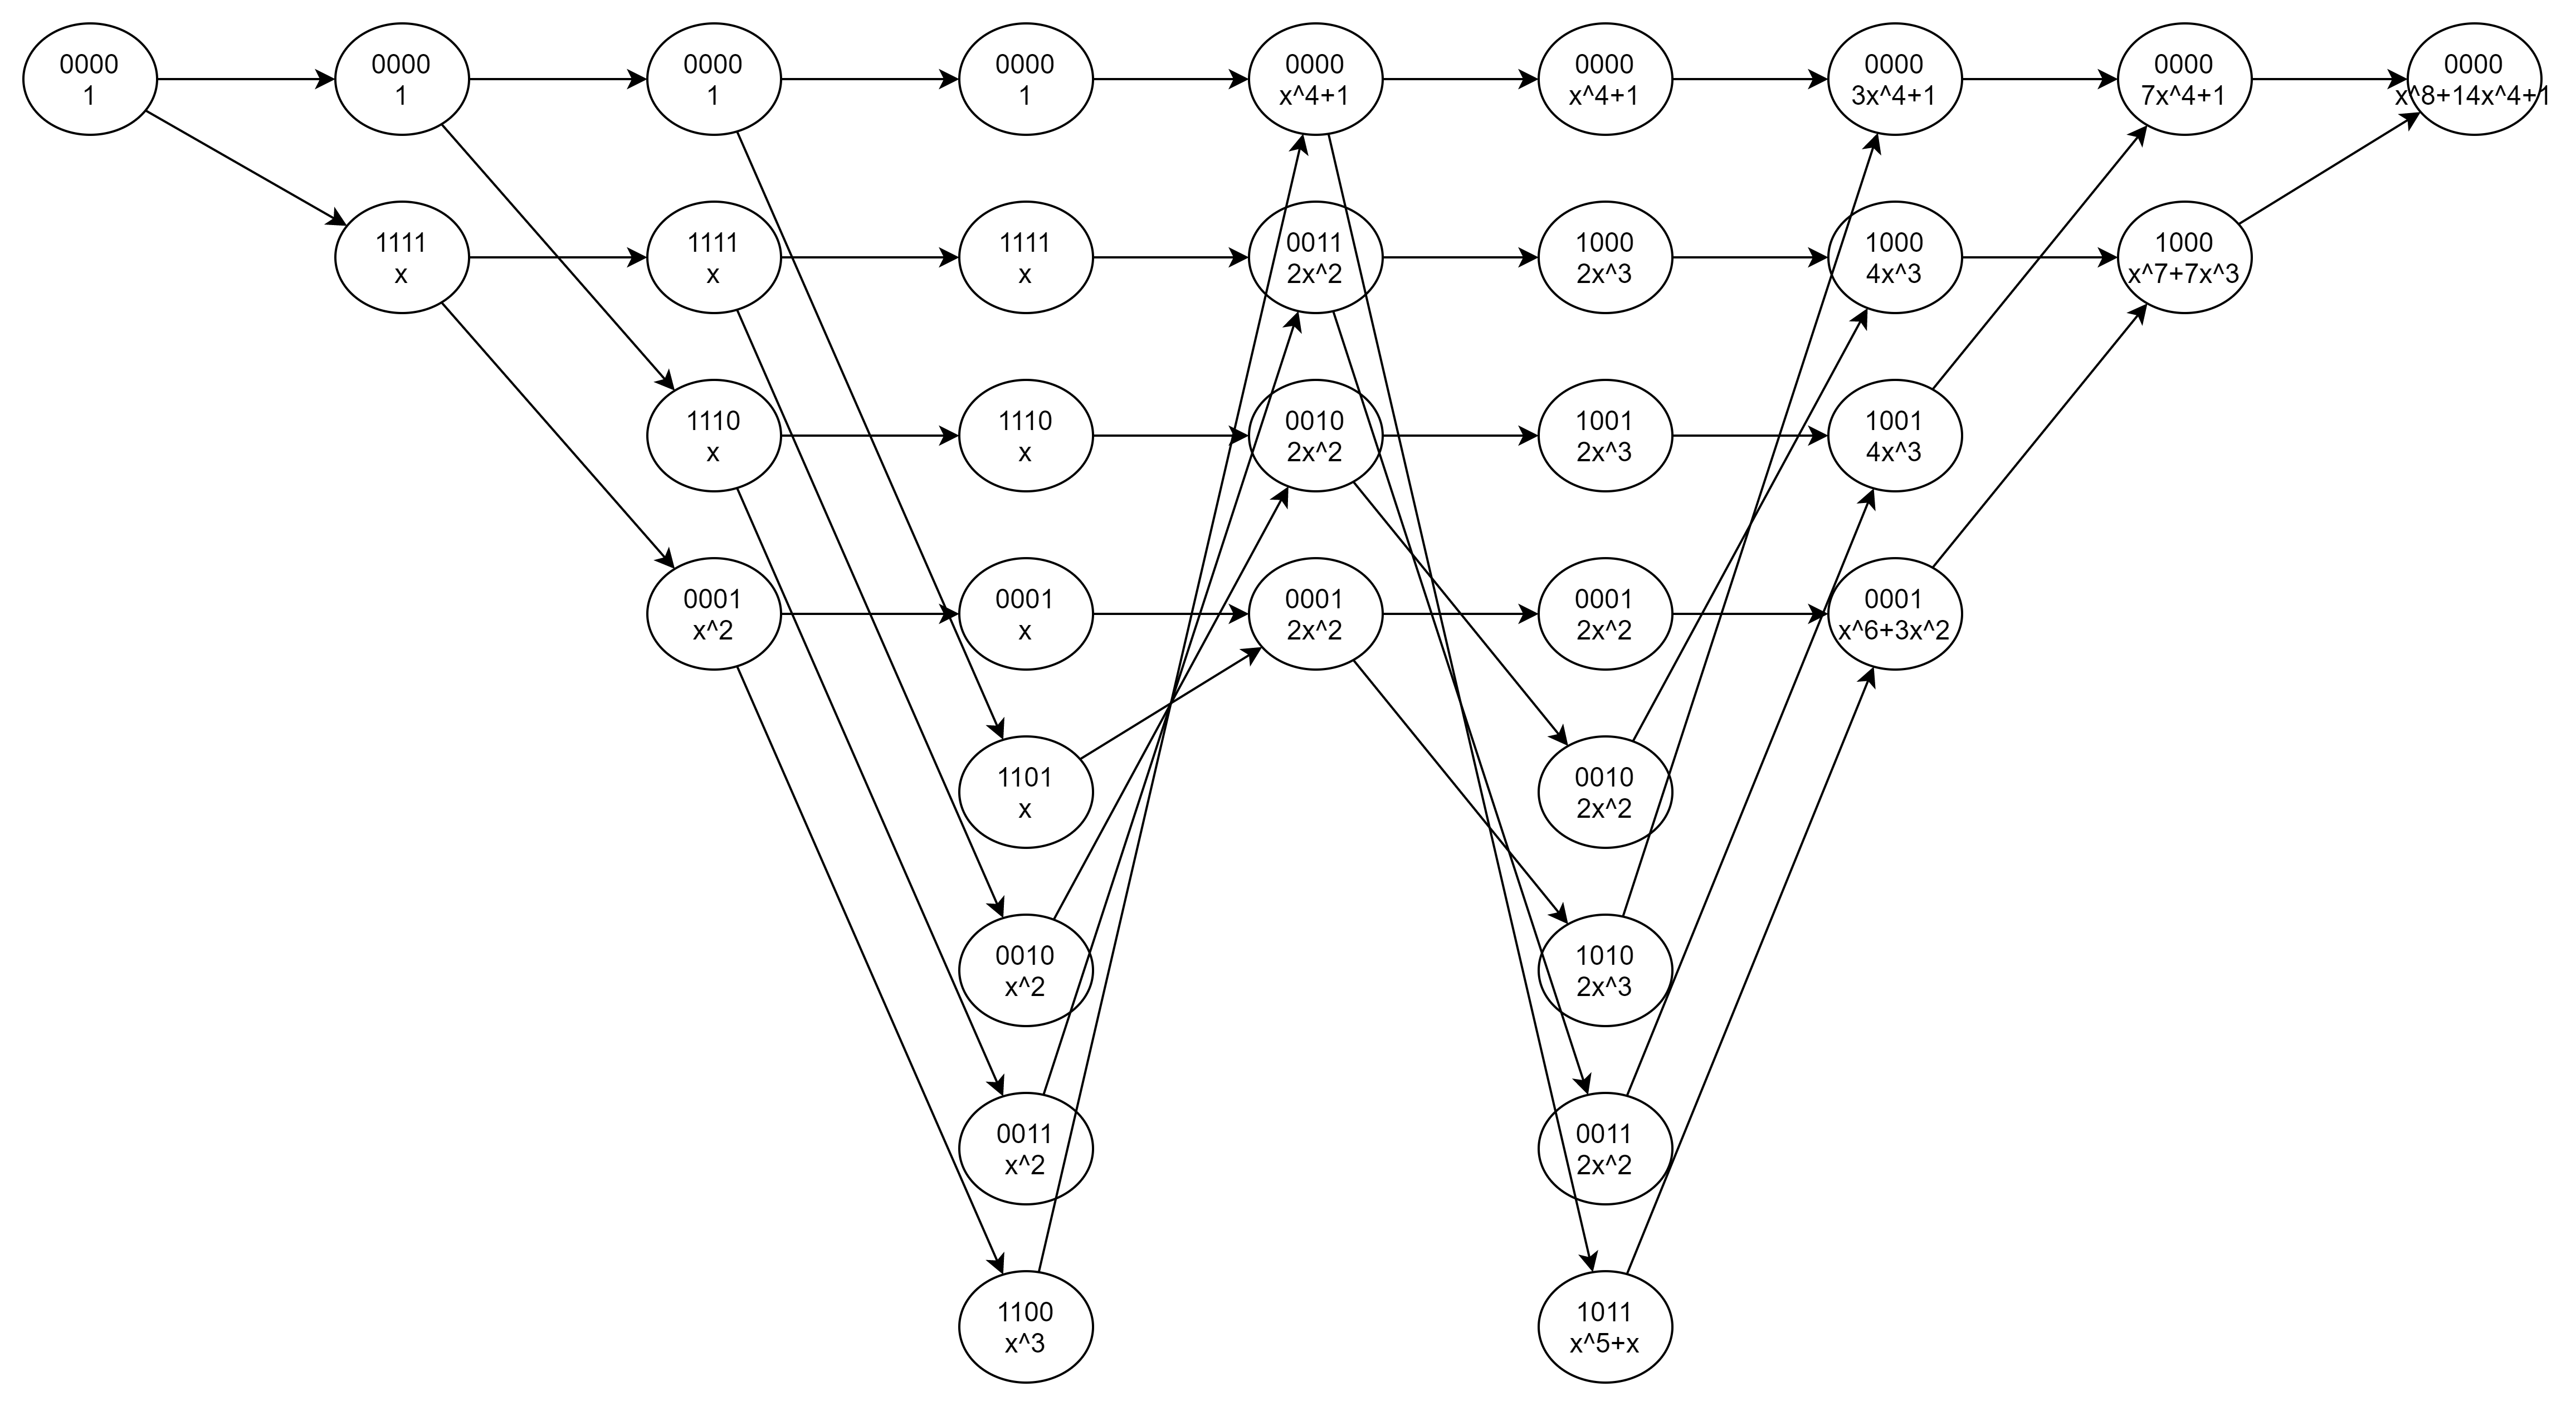
\includegraphics[width=1.5\textwidth,center]{resources/lattice.png}
    \caption{Решётка для проверочной матрицы}
    \label{fig:mesh1}
\end{figure}

\subsection*{Профиль решётки}

Профиль решётки --- это такая последовательность чисел $\{s_n\}$,\\ что $s_i = \lfloor\log_2{C_i}\rfloor$, где $C_i$ --- число вершин на $i$-м уровне этой решётки. Например, для рёшетки из предыдущего примера, профиль будет равен $\{0, 1, 2, 3, 2, 3, 2, 1, 0\}$.

Также можно вычислить, что количество операций в алгоритме Витерби в зависимости от профиля решётки составляет $O(\sum 2^{s_i})$.

\end{document}
